\section{Sistema propuesto}
Para este proyecto se planteó un sistema que implementa un control de FES en lazo cerrado utilizando la técnica de biofeedback. El sistema consiste en la adquisición de dos canales de sEMG, del brazo izquierdo, los cuales son procesados y se utilizan como entrada de un sistema de control que realiza la modulación de la amplitud de dos canales de estimulación eléctrica en el brazo derecho. Este sistema implementa un control contralateral para realizar un entrenamiento en espejo de las acciones de apertura y cierre de mano.

En la Figura \ref{Figura: SistProp} se muestra un esquema general del sistema desarrollado, en el cual se muestran en rojo los elementos implementados en este proyecto.

%Sistema propuesto
\begin{figure}[htbp]
\centering
	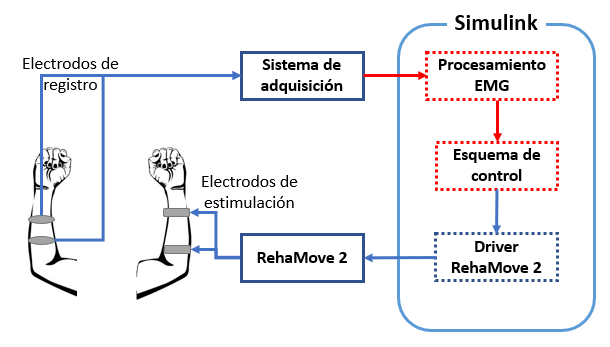
\includegraphics[scale=0.7]{SistemaPropuesto.png}
	\caption[Sistema propuesto para el proyecto]{Sistema propuesto para el proyecto. Líneas continuas representan entes de hardwares y líneas discontinuas representan entes de software. Elementos en rojo representan zonas de trabajo del proyecto.}
	\label{Figura: SistProp}
\end{figure}


\section{Adquisición de datos en Simulink}
Se utilizó el sistema Cyton Board, el cual tiene una frecuencia de muestreo de 250 Hz, para realizar la adquisición de las señales de sEMG. Dicho sistema utiliza un chip ADS1299 (Texas Instruments Inc., Dallas, E.U.A.) para realizar la conversión analógico-digital de las señales, el cual codifica los datos de cada muestra, utilizando complemento a 2, en un flujo de datos de 27 bytes esquematizado en la Figura \ref{Figura: BusOut}.

%Stream datos ADS
\begin{figure}[htbp]
\centering
	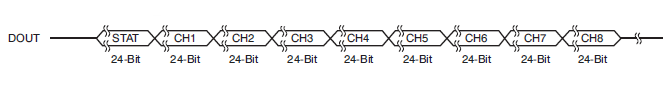
\includegraphics[scale=0.8]{Bus_Dat_Out_ADS.png}
	\caption{Flujo de datos de salida del ADS1299.}
	\label{Figura: BusOut}
\end{figure}

Para realizar la decodificación del flujo de datos dentro de Simulink, se diseñó un subsistema encargado de la solicitud y decodificación de datos, para esto se utilizó el bloque \emph{Query Instrument} del \emph{Instrument Control Toolbox} para realizar la solicitud de datos, los cuales fueron decodificados con bloques de la librería estándar de Simulink. La figura \ref{Figura: DecoSimuT} muestra la implementación dentro de Simulink del sistema antes mencionado.

\hfill \break

%Sistema Simulink
\begin{figure}[htbp]
	\centering
	\begin{subfigure}[htbp]{0.8\textwidth}
		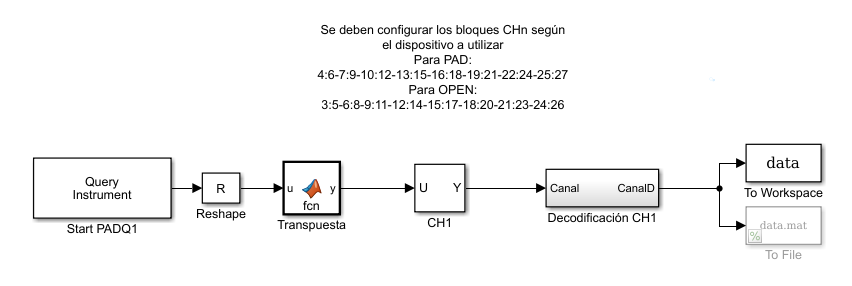
\includegraphics[width=\textwidth]{Read_Simu.png}
		\caption{Vista general del subsistema diseñado para realizar adquisición y decodificación del flujo de datos.}
		\label{Figura: readSimu}
	\end{subfigure}
	\begin{subfigure}[htbp]{0.8\textwidth}
		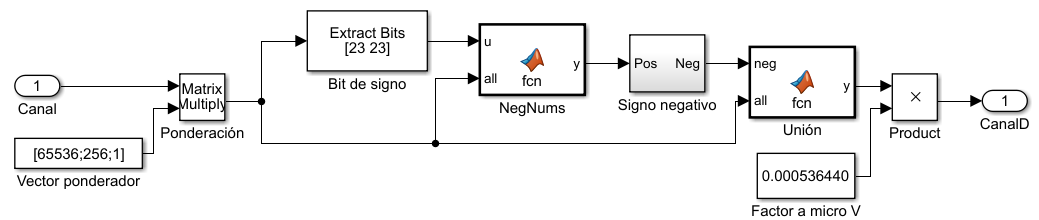
\includegraphics[width=\textwidth]{Deco_Simu.png}
		\caption{Vista interna del subsistema encargado de la decodificación del flujo de datos.}
		\label{Figura: decoSimu}
	\end{subfigure}
	\caption[Subsistema decodificador del flujo de datos]{Subsistema decodificador del flujo de datos implementado en Simulink.}
	\label{Figura: DecoSimuT}
\end{figure}

\newpage
El funcionamiento del subsistema responsable de la solicitud y decodificación de datos implementado dentro de Simulink se encuentra esquematizado en la Figura \ref{Figura: DecoStream}, y lleva a cabo el siguiente algoritmo:

\begin{enumerate}
	\item Se realiza la adquisición de N muestras, lo cual generará un vector columna con dimensión $\mathbb{R}^{27*N\times 1}$ (Figura \ref{Figura: DecoStream} \emph{(a)}).
	\item Se aplicar un reshape a dicho vector para obtener una matriz con dimensión $\mathbb{R}^{27\times N}$ (Figura \ref{Figura: DecoStream} \emph{(b)}).
	\item Se obtiene la transpuesta de dicha matriz para obtener una matriz con dimension $\mathbb{R}^{N\times 27}$ (Figura \ref{Figura: DecoStream} \emph{(c)}).
	\item Se realiza la extracción de las columnas asociadas al canal a procesar, obteniendo una matriz con dimensión $\mathbb{R}^{N\times 3}$ (Figura \ref{Figura: DecoStream} \emph{(d)}).
	\item Se realiza el producto matricial de la matriz del canal a procesar con un vector ponderador que contiene el peso de cada columna (byte) para el valor de la muestra de 24 bits (Figura \ref{Figura: DecoStream} \emph{(e)}). El vector ponderador está compuesto por los valores $2^{16}$, $2^8$, $1$. Como resultado de dicho producto se obtiene un vector de dimensión $\mathbb{R}^{N\times 1}$ (Figura \ref{Figura: DecoStream} \emph{(f)}).
	\item Se extraen del vector anterior las muestras en las que se encuentren codificados, en complemento a 2, un número negativo. Esto se realiza al obtener el valor del bit 23 (bit más significativo), y si dicho bit tiene un valor de 1 implica que dicha muestra codifica un número negativo (Figura \ref{Figura: DecoStream} \emph{(g)}).
	\item Se obtiene el complemento a 1 de cada muestra del vector \emph{g}, se suma 1 a cada muestra y se multiplica cada muestra por -1. De esta operación se obtiene un vector con las muestras decodificadas a número negativos (Figura \ref{Figura: DecoStream} \emph{(h)}).
	\item Se insertan los elementos del vector \emph{h} en sus posiciones originales del vector \emph{f}. De este último paso se obtiene un vector con las N muestras decodificadas a números de 24 bits con signo (Figura \ref{Figura: DecoStream} \emph{(i)}).
\end{enumerate}

%Funcionamiento decodificación
\begin{figure}[htbp]
\centering
	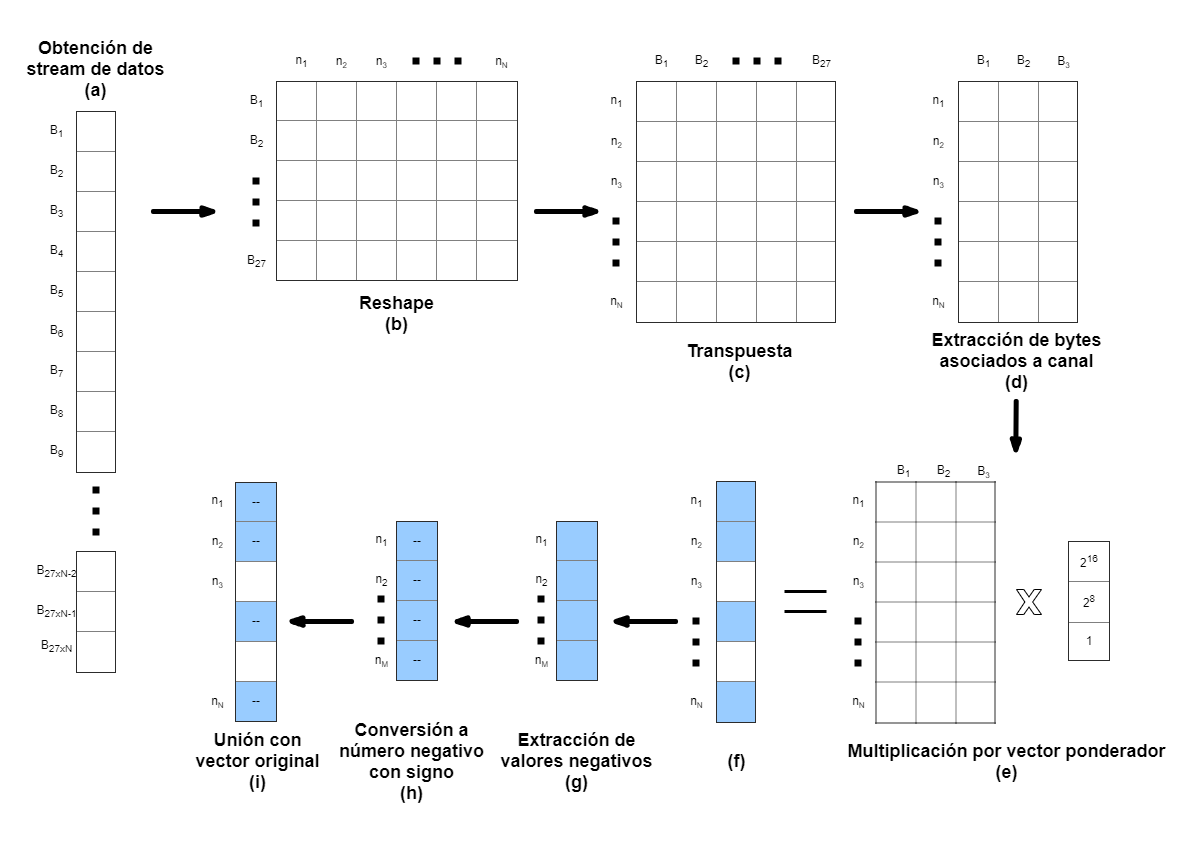
\includegraphics[width=\textwidth]{DecoStream.png}
	\caption{Funcionamiento del subsistema decodificador del flujo de datos.}
	\label{Figura: DecoStream}
\end{figure}


\newpage
\section{Evaluación de bloque de adquisición y decodificación}
Se llevó a cabo un procedimiento para evaluar el desempeño del subsistema diseñado en Simulink para la adquisición y decodificación de datos. En MATLAB se generó un banco de señales senoidales conformado por 5 senoidales puras de 1 Hz, 5 Hz, 10 Hz, 20 Hz y 50 Hz (\ref{Figura: SenPur}), dos senoidales de 50 Hz moduladas en amplitud con una envolvente de una recta con pendiente negativa (\ref{Figura: LinAte}) y una exponencial decreciente (\ref{Figura: ExpAte}), y una senoidal de 50 Hz modulada en amplitud con una envolvente que simula la señal sEMG correspondiente a la tarea de incrementar gradualmente una contracción muscular, mantener dicha contracción y relajar el músculo gradualmente (\ref{Figura: Contra}). Todas las señales del banco se diseñaron con una frecuencia de muestreo de 250 Hz y una duración de 5 segundos, excepto la última, que se diseñó con una duración de 15 segundos; adicionalmente, todas las señales se generaron como objetos de audio dentro de MATLAB, para poder reproducirlas como audio y a partir de la salida de audio de la computadora poder acceder a ellas.

%Figura de senoidales MATLAB
\begin{figure}[htbp]
	\centering
	\begin{subfigure}[htbp]{0.45\textwidth}
		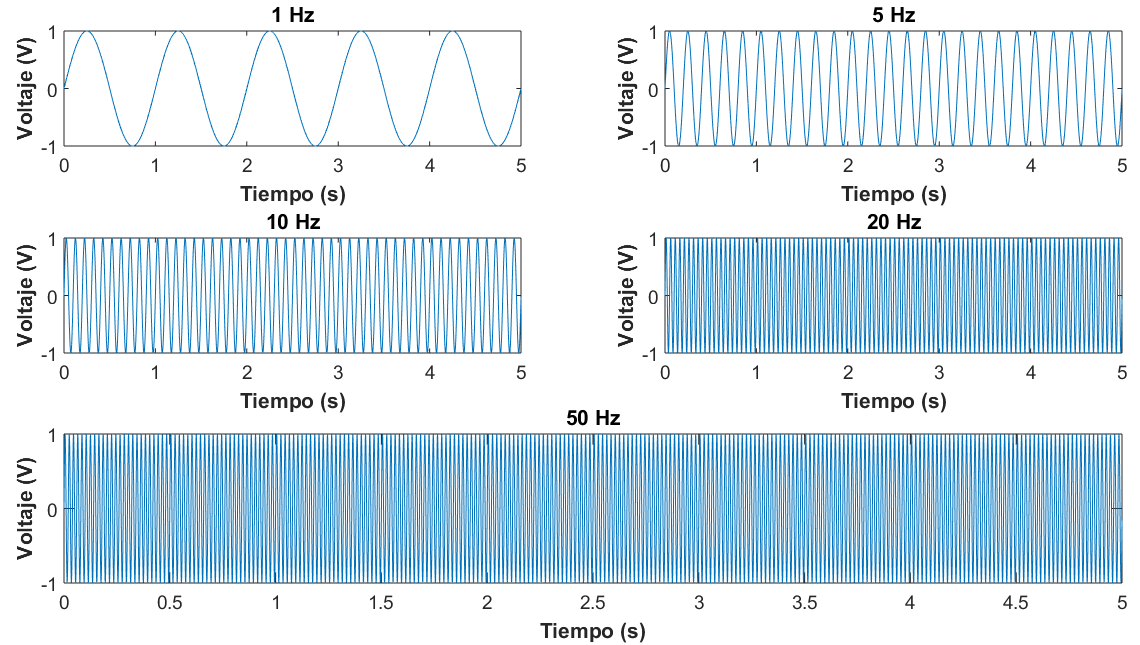
\includegraphics[width=\textwidth]{Sen_Pur.png}
		\caption{Senoidales puras a diferentes frecuencias.}
		\label{Figura: SenPur}
	\end{subfigure}
	\hfill
	\begin{subfigure}[htbp]{0.45\textwidth}
		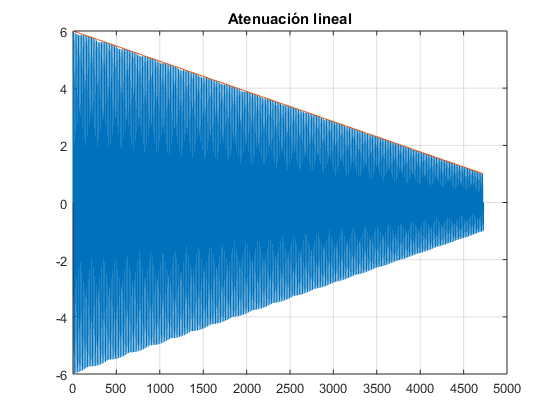
\includegraphics[width=\textwidth]{Lin_Ate.png}
		\caption{Senoidal de 50 Hz con atenuación lineal.}
		\label{Figura: LinAte}
	\end{subfigure}
	\hfill
	\begin{subfigure}[htbp]{0.45\textwidth}
		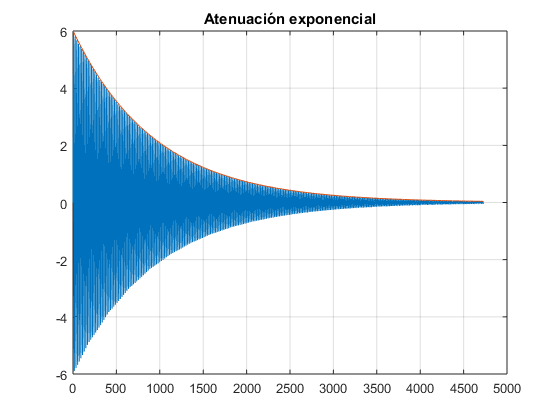
\includegraphics[width=\textwidth]{Exp_Ate.png}
		\caption{Senoidal de 50 Hz con atenuación exponencial.}
		\label{Figura: ExpAte}
	\end{subfigure}
	\hfill
	\begin{subfigure}[htbp]{0.45\textwidth}
		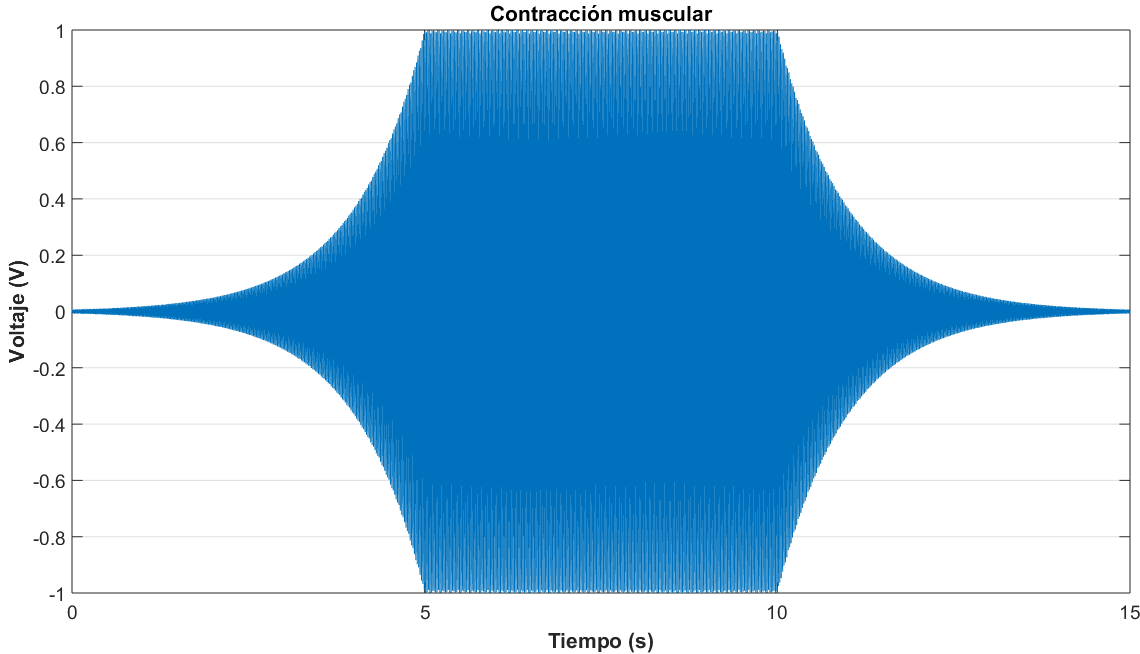
\includegraphics[width=\textwidth]{Contra.png}
		\caption{Senoidal de 50 Hz simulando el sEMG de una contracción muscular.}
		\label{Figura: Contra}
	\end{subfigure}	
	\caption{Banco de señales para evaluación de adquisición.}
	\label{Figura: SenalesEva}
\end{figure}

\newpage
El proceso para la evaluación del funcionamiento del subsistema de adquisición se llevó a cabo de la siguiente manera:
\begin{enumerate}
	\item Se realiza la adquisición de tres tantos de todas las señales del banco de señales de prueba.
	\begin{enumerate}
		\item Se conecta una punta de un jack de audio de 3.5 mm a la salida de audio de la computadora. La otra punta se conectó al dispositivo de adquisición (Cyton Board) de la siguiente forma: el pin \emph{izquierdo} se conectó a un pin diferencial del canal 1, mientras que el pin \emph{tierra} se conectó a la entrada BIAS y al pin diferencial restante del canal 1. La Figura \ref{Figura: JackConexion} ilustra estas conexiones.
		\item Se realiza la solicitud de datos utilizando el subsistema decodificador implementado en Simulink, y al mismo tiempo se inicia el conteo de un cronómetro.
		\item Tras haber transcurrido 2 s en el cronómetro, se procede a reproducir la señal de audio de prueba.
		\item Tras haber transcurrido 10 s (20 s para la simulación del sEMG de una contracción), se detiene la adquisición del subsistema de Simulink y se guardan los datos de adquisición dentro de un archivo con extensión \emph{.mat}.
	\end{enumerate}
	\item Se cargan, dentro del workspace de MATLAB, los datos de las señales adquiridas y los datos de las señales patrón.
	\item Se procede a calcular el coeficiente de correlación de Pearson (Ecuación \ref{Ecu: CorrePea}) entre las señales adquiridas y su correspondiente señal patrón.
	\item Se obtiene la media aritmética de todos los valores obtenidos al aplicar el coeficiente de correlación de Pearson. El valor obtenido se utiliza como indicador de la calidad del subsistema de adquisición y decodificación de datos.
\end{enumerate}

%Ecuación correlación Pearson
\begin{equation}
	r = \frac{\sigma_{xy}}{\sigma_{x}\sigma_{y}}
	\label{Ecu: CorrePea}
\end{equation}

\begin{figure}
	\centering
	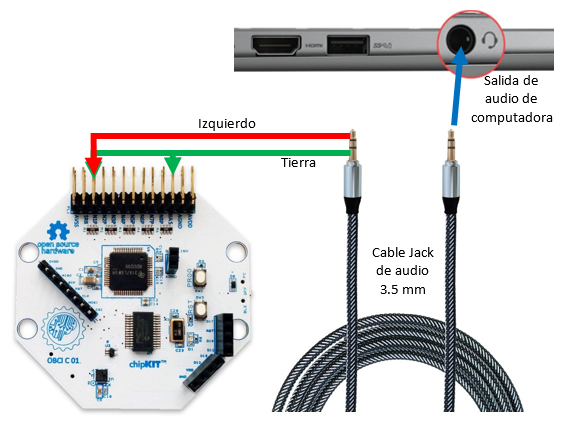
\includegraphics[width=0.5\textwidth]{JackConexion.png}
	\caption{Conexiones para evaluación de bloque de adquisición.}
	\label{Figura: JackConexion}
\end{figure}

\newpage
\section{Protocolo para registro de sEMG}\label{Section: ProReg}
Para garantizar repetibilidad en los registros de sEMG se implementó un protocolo para realizar la adquisición de dicha señal. Dicho protocolo se describe a continuación y utiliza electrodos Telectrode T718 (Bio-Protech Inc., Chino, E.U.A.):

\begin{enumerate}
	\item Se configura el dispositivo de adquisición (Para el caso del Cyton Board esta configuración es la default):
	\begin{enumerate}
		\item Frecuencia de muestreo a 250 Hz.
		\item Ganancia 24 para los canales de adquisición 1 y 2.
		\item BIAS habilitado para los canales de adquisición 1 y 2.
	\end{enumerate}
	\item Se prepara la zonas donde se colocaran los electrodos, limpiando con algodón y alcohol las zonas ventral y dorsal del antebrazo, así como el codo.
	\item Se ubican los puntos para colocación de electrodos:
	\begin{enumerate}
		\item Para músculo flexor digitorum (\ref{Figura: E_Cie}):
		\begin{enumerate}
			\item Se mide la distancia de codo a muñeca en el lado ventral del antebrazo.
			\item Se coloca una marca al 25\% de la medida obtenida.
		\end{enumerate}
		\item Para músculo extensor digitorum (\ref{Figura: E_Ape}):
		\begin{enumerate}
			\item Se mide la distancia de codo a muñeca en el lado dorsal del antebraz.
			\item Se coloca una marca al 75\% de la medida obtenida.
		\end{enumerate}
	\end{enumerate}
	\item Se colocan, sobre la marca obtenida para el flexor digitorum (\ref{Figura: E_Cie}), dos electrodos (en dirección de la fibra muscular) separados 3 cm. Dicho par de electrodos se conecta al canal 1 del dispositivo de adquisición.
	\item Se colocan, sobre la marca obtenida para el extensor digitorum (\ref{Figura: E_Ape}), dos electrodos (en dirección de la fibra muscular) separados 3 cm. Dicho para de electrodos se conecta al canal 2 del dispositivo de adquisición.
	\item Se coloca un electrodo de referencia sobre el codo. Dicho electrodo se conecta al BIAS del dispositivo de adquisición.
\end{enumerate}

%Ubicación electrodos
\begin{figure}[htbp]
	\centering
	\begin{subfigure}[htbp]{0.3\textwidth}
		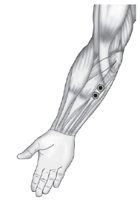
\includegraphics[width=\textwidth]{E_Cie.png}
		\caption{Ubicación de electrodos para flexor digitorum.}
		\label{Figura: E_Cie}
	\end{subfigure}
%	\hfill
	\hspace{3cm}
	\begin{subfigure}[htbp]{0.3\textwidth}
		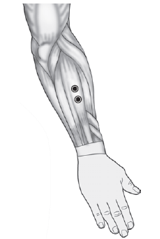
\includegraphics[width=\textwidth]{E_Ape.png}
		\caption{Ubicación de electrodos para extensor digitorum.}
		\label{Figura: E_Ape}
	\end{subfigure}
	\caption[Posicionamiento de electrodos para registro de sEMG]{Posicionamiento de electrodos para realizar registros de sEMG. Adaptado de \cite{Cavalcanti-Garcia2009}.}
	\label{Figura: E_sEMG}
\end{figure}


\section{Procesamiento de sEMG}
Se diseñaron tres filtros digitales Butterworth orden 2 para realizar el procesamiento de sEMG: un filtro pasa altas con frecuencia de corte de 15 Hz, para eliminar las variaciones en la línea base del registro; un filtro pasa bajas con frecuencia de corte de 100 Hz, para eliminar armónicos de 60 Hz y demás interferencias de alta frecuencia; y un filtro rechaza banda centrado en 60 Hz, para reducir la interferencia de la línea. Todos estos filtros se diseñaron utilizando la función \emph{butter} de MATLAB. Las gráficas de respuesta en frecuencia de estos filtros se muestran en las Figuras \ref{Figura: FiltroPA} a \ref{Figura: FiltroRB}.

%Respuesta en frecuencia de filtros
\begin{figure}[htbp]
	\centering
	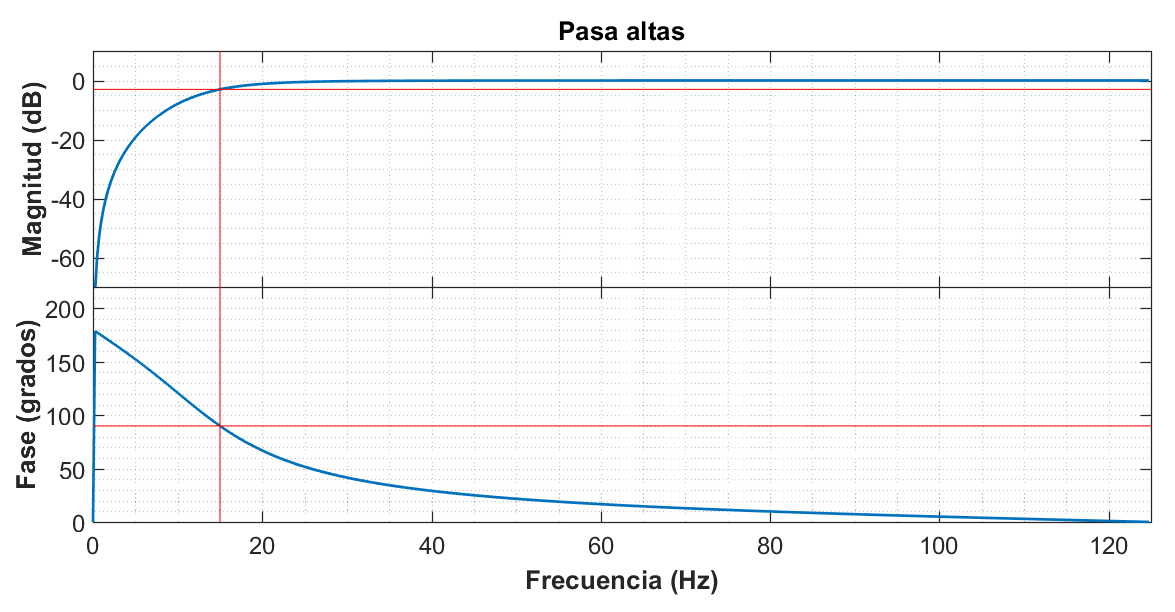
\includegraphics[width=0.7\textwidth]{FiltroPA15Hz_PADQ.png}
	\caption{Respuesta en frecuencia de filtro pasa altas.}
	\label{Figura: FiltroPA}
	
	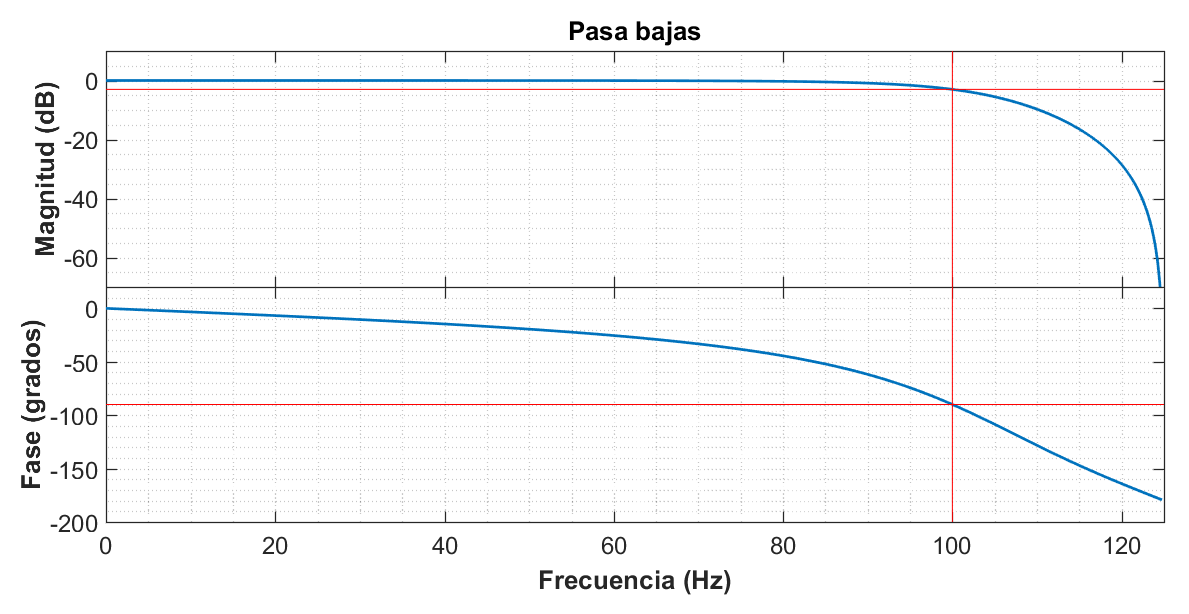
\includegraphics[width=0.7\textwidth]{FiltroPB100Hz_PADQ.png}
	\caption{Respuesta en frecuencia de filtro pasa bajas.} 
	\label{Figura: FiltroPB}
	
	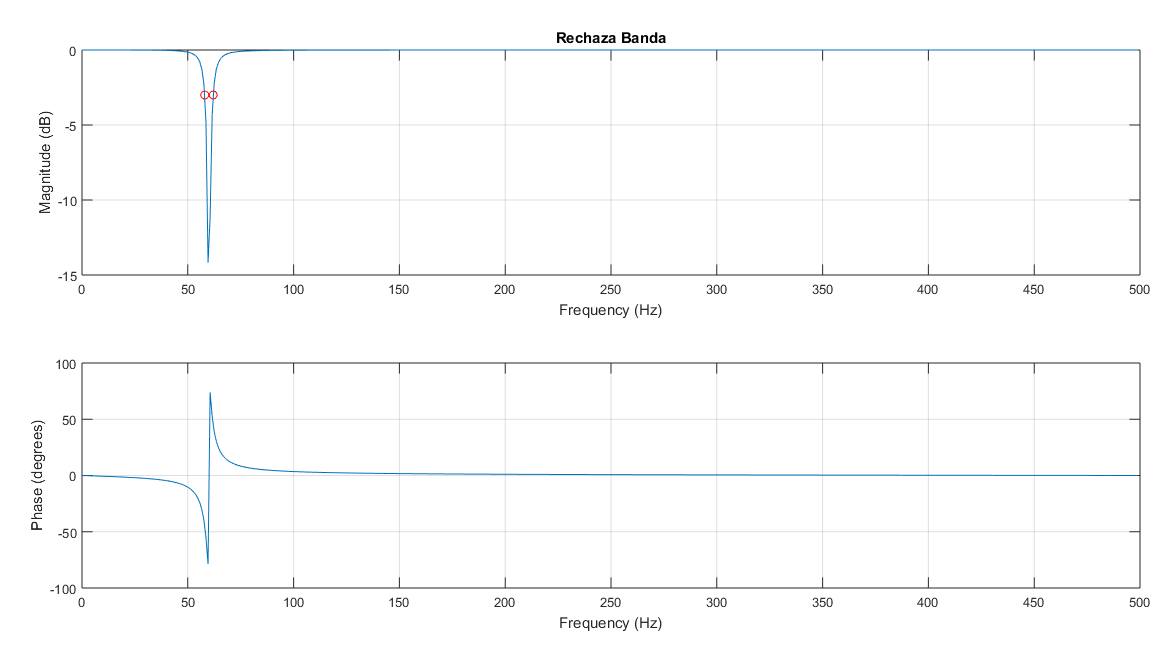
\includegraphics[width=0.7\textwidth]{FiltroRB_58_62_PADQ.png}
	\caption{Respuesta en frecuencia de filtro rechaza banda.}
	\label{Figura: FiltroRB}
\end{figure}

Se implementó dentro de Simulink un bloque responsable de obtener el valor RMS de ventanas de 100 ms del registro de sEMG, para utilizar dicho descriptor de amplitud como señal de control. Adicionalmente se implementó un filtro de mediana de 10 muestras (Ecuación \ref{Ecu: Mediana}), el cual tiene como propósito conseguir una señal de RMS suavizada.

%Ecuación filtro mediana
\begin{equation}
	y[n] = mediana(x[n]:x[n-N])
	\label{Ecu: Mediana}
\end{equation}


\newpage
\section{Sistema de control}
A grandes rasgos, el sistema de control implementado para este proyecto consta de la combinación de una FSM y un control proporcional. La FSM (Figura \ref{Figura: FSM_Control}) permite clasificar la intención de movimiento del sujeto en tres clases (descanso, pinza gruesa y apertura), mientras que el control proporcional permite realizar la modulación de la amplitud de corriente eléctrica a partir de la amplitud del sEMG.

%FSM
\begin{figure}[htbp]
	\centering
	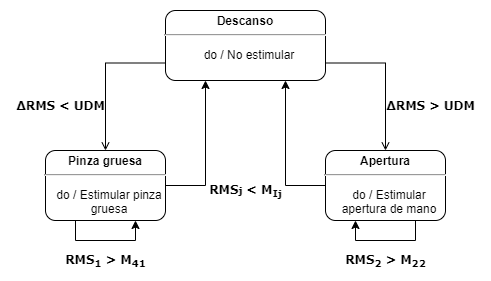
\includegraphics[scale=0.7]{FSM_Control.png}
	\caption[FSM para control]{Máquina de estados finitos encargada de la detección de movimiento e inicio del control proporcional.}
	\label{Figura: FSM_Control}
\end{figure}

La máquina de estados necesita principalmente tres parámetros para llevar a cabo la clasificación de los movimientos: detector de movimiento ($DM$), umbral de pinza gruesa incompleta ($M_{1I}$) y umbral de apertura de mano incompleta ($M_{2I}$), y dentro de los estados pinza gruesa y apertura, la FSM necesita de la ecuación de control proporcional para poder llevar a cabo la modulación de la estimulación eléctrica. La obtención de dichos parámetros se obtiene de un proceso de calibración que se realiza para cada sesión de prueba.

Posterior al proceso de calibración se realiza una validación fuera de línea, donde a partir del registro de calibración y los parámetros arrojados por esta se pone a prueba el funcionamiento del sistema. Cuando la validación fuera de línea presenta un porcentaje de acierto igual o mayor al 80$\%$ se procede a configurar el sistema para realizar una prueba en línea y posteriormente realizar la tarea objetivo.

Todas las etapas antes mencionadas por las que se somete el sistema de control se describen a continuación.

\subsection{Calibración}
El proceso de calibración del sistema consta a su vez de una calibración de los parámetros de estimulación eléctrica y una calibración de los valores de amplitud RMS del sEMG.

\subsubsection{Calibración de parámetros FES}
El objetivo de esta calibración es el obtener los umbrales motores y funcionales de los movimientos de apertura de mano y pinza gruesa. Para esta calibración se utiliza el sistema de colocación de electrodos de estimulación eléctrica desarrollado en el INR-LGII, el cual se encuentra descrito en \cite{AnaMartin2019}, en conjunto con la pantalla \emph{Experimentación} (Figura \ref{Figura: GUI_Exp}) de la GUI diseñada en el INR-LGII \cite{JanethFuentes2018}.

El proceso para la obtención de los umbrales antes mencionados consiste en realizar la colocación de los electrodos de estimulación eléctrica y realizar una exploración de la respuesta del sujeto ante diferentes valores de amplitud de corriente eléctrica que le serán proporcionados. Dichos valores exploran el rango entre 1 y 15 mA, utilizando un incremento de 1 mA. El umbral motor será el primer valor de amplitud que genere una respuesta motora en la mano del sujeto; mientras que el umbral funcional será aquél valor de amplitud en el que la respuesta motora en la mano del sujeto sea similar al movimiento que se está calibrando.

%Experimentación
\begin{figure}[htb]
	\centering
	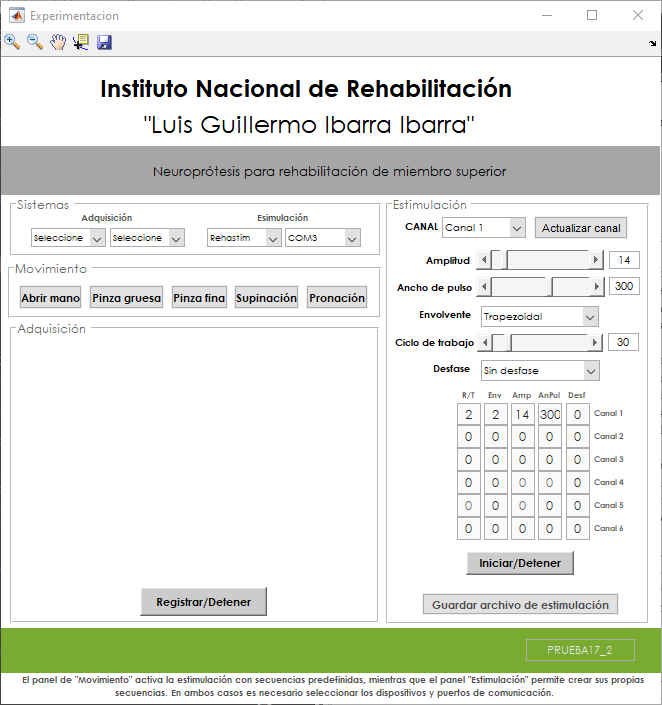
\includegraphics[width=0.6\textwidth]{GUI_Exp.png}
	\caption{Pantalla utilizada para calibración de FES.}
	\label{Figura: GUI_Exp}
\end{figure}

\subsubsection{Calibración de amplitud RMS de sEMG}
Para realizar esta calibración se utiliza el protocolo de registro descrito en la sección \ref{Section: ProReg} y una pantalla de calibración diseñada para este proyecto (Figura \ref{Figura: GUI_Ent}), la cual muestra indicaciones de los movimientos que debe realizar el sujeto y a la par realiza el registro de sEMG. Una vez colocados los electrodos para registro de sEMG, se le muestra al sujeto cuales son los movimientos asociados a cada una de las indicaciones que se le irán mostrando en la GUI. Los movimientos mostrados son denominados \emph{descanso} (DD), \emph{apertura incompleta} (AI), \emph{apertura completa} (AC), \emph{pinza gruesa incompleta} (CI) y \emph{pinza gruesa completa} (CC), los cuales se pueden observar en la Figura \ref{Figura: Posturas}.

Al terminar las repeticiones de los movimientos solicitados, la GUI nos arroja en la consola de MATLAB los valores de los umbrales RMS para los movimientos apertura de mano incompleta y completa, pinza gruesa incompleta y completa, y descanso, para cada canal de registro. La obtención de estos umbrales se realiza mediante la Ecuación \ref{Ecu: U_RMS}, donde $M_i$ representa a uno de los 5 movimientos antes mencionados, $RMS_n$ representa al valor RMS obtenido para la n-esima ventana de registro (100 ms) asociada al movimiento $M_i$, y $N$ representa la cantidad de valores RMS asociados al movimiento $M_i$.

%Ecuación obtención de umbrales
\begin{equation}
	M_i = \frac{\sum_{n=1}^{N}RMS_{n}}{N}
	\label{Ecu: U_RMS}
\end{equation}

La GUI también proporciona un valor denominado \emph{detector de movimiento} (DM), y los parámetros de las rectas que se utilizarán para llevar a cabo el control lineal.

El detector de movimiento, junto a los umbrales de movimiento incompleto, se utiliza para llevar a cabo la transición de estados de la FSM, siendo esta última la encargada de clasificar la intención de movimiento del sujeto. El detector de movimiento se obtiene utilizando la Ecuación \ref{Ecua: DM}, donde $RMS_{2n}$ y $RMS_{1n}$ representan el valor RMS de la n-esima ventana de registro para el movimiento de apertura incompleta en los canales 2 y 1 respectivamente, y $N$ representa la cantidad de valores RMS existentes para el movimiento de apertura incompleta.

%Ecuación detector movimiento
\begin{equation}
	DM = \frac{\sum_{n=1}^{N}RMS_{2n}-RMS_{1n}}{N}
	\label{Ecua: DM}
\end{equation}

Los parámetros de las rectas que arroja la GUI son la pendiente (m) y la ordenada al origen (b), donde dichas rectas son utilizadas para llevar a cabo el control lineal de los movimientos apertura de mano y pinza gruesa. Estos parámetros se obtienen a partir de las Ecuaciones \ref{Ecu: m} y \ref{Ecu: b}, donde $m_{i}$ y $b_{i}$ representan la pendiente y ordenada al origen, respectivamente, de la i-esima recta; $U_{iF}$ y $U_{iM}$ representan los umbrales funcionales y motores, respectivamente, obtenidos tras la calibración de parámetros FES para el i-esimo movimiento correspondiente; $M_{iC}$ y $M_{iI}$ representan los umbrales de los movimientos completos e incompletos, respectivamente, del i-esimo canal de registro.

%Ecuación pendiente
\begin{equation}
	m_{i} = \frac{ U_{iF} - U_{iM} }{ M_{iC} - M_{iI} }
	\label{Ecu: m}
\end{equation}

%Ecuación ordenada
\begin{equation}
	b_{i} = U_{iM} - m_{i}*M_{iI}
	\label{Ecu: b}
\end{equation}

%Entrenamiento_sEMG
\begin{figure}[htb]
	\centering
	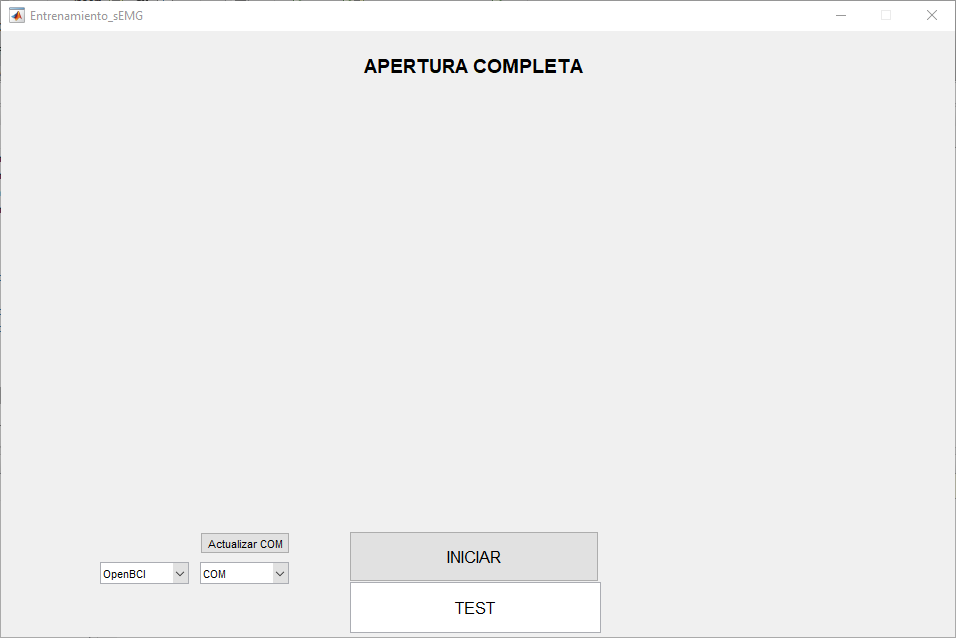
\includegraphics[width=0.7\textwidth]{GUI_Ent.png}
	\caption{GUI utilizada para calibración de amplitud RMS.}
	\label{Figura: GUI_Ent}
\end{figure}

%Posturas manos
\begin{figure}[htbp]
	\centering
	\begin{subfigure}[htbp]{0.4\textwidth}
		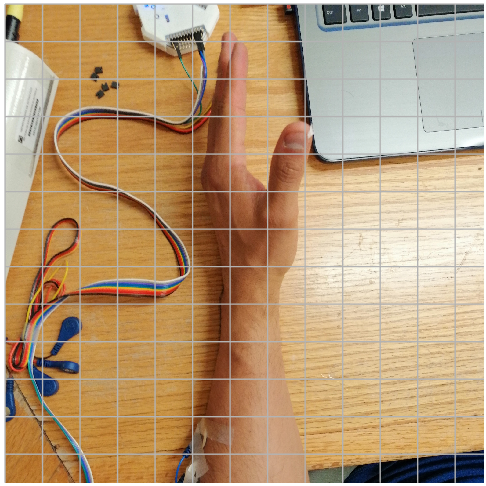
\includegraphics[width=\textwidth]{AI_g.png}
		\caption{Apertura incompleta.}
		\label{Figura: AI}
	\end{subfigure}
%	\hfill
	\begin{subfigure}[htbp]{0.4\textwidth}
		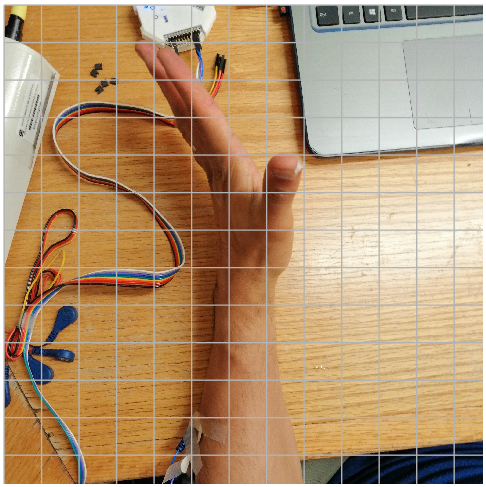
\includegraphics[width=\textwidth]{AC_g.png}
		\caption{Apertura completa.}
		\label{Figura: AC}
	\end{subfigure}
%	\hfill
	\newline
	\begin{subfigure}[htbp]{0.4\textwidth}
		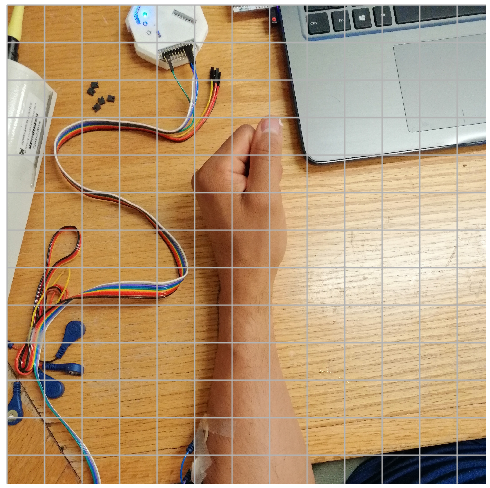
\includegraphics[width=\textwidth]{CI_g.png}
		\caption{Pinza gruesa incompleta.}
		\label{Figura: CI}
	\end{subfigure}
%	\hfill
	\begin{subfigure}[htbp]{0.4\textwidth}
		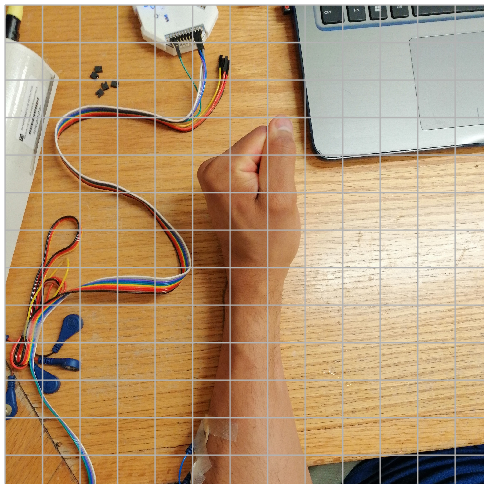
\includegraphics[width=\textwidth]{CC_g.png}
		\caption{Pinza gruesa completa.}
		\label{Figura: CC}
	\end{subfigure}
%	\hfill
	\newline
	\begin{subfigure}[htbp]{0.4\textwidth}
		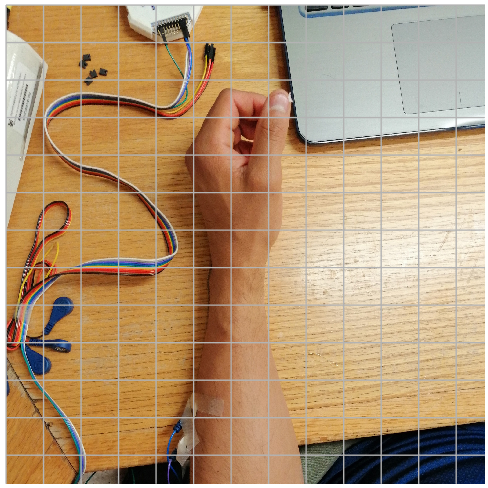
\includegraphics[width=\textwidth]{DD_g.png}
		\caption{Descanso.}
		\label{Figura: DD}
	\end{subfigure}
	\caption[Posturas de mano para calibración]{Posturas de mano para calibración. Se agregó una cuadrícula a la imagen para poder observar las diferencias entre una postura y otra.}
	\label{Figura: Posturas}
\end{figure}

\subsection{Validación fuera de línea}
El propósito de esta prueba consiste en obtener un indicador que proporcione información sobre el desempeño del sistema, al configurarlo con los parámetros obtenidos en la calibración, en su función de clasificación de movimientos.

Para obtener dicho indicador, se diseñó un script en MATLAB que lee el registro de sEMG crudo obtenido en la etapa de calibración, posteriormente le aplica una etapa de procesamiento (filtrado, obtención de RMS y suavizado) y por último aplica el algoritmo de control diseñado (FSM y control proporcional); una vez obtenida la salida del algoritmo de control, se procede a realizar el conteo de los errores y aciertos que tuvo el sistema al realizar la clasificación de los movimientos, expresando dichos valores en términos de porcentaje. Si el porcentaje obtenido de acierto es igual o mayor al 80$\%$, se procede a configurar el sistema diseñado en Simulink con los parámetros arrojados en la calibración, en caso contrario, se revisa si existen problemas en la colocación de electrodos para registro de sEMG y se repite el proceso de calibración.

\newpage
\subsection{Validación en línea}
Una vez que el sistema se ha validado fuera de línea, se procede a realizar una prueba para corroborar su funcionamiento en línea. Para esto, se configura el bloque \emph{Control} del sistema completo implementado en Simulink (Figura \ref{Figura: SisComp}) con los parámetros obtenidos en la calibración, posteriormente, se configura el switch \emph{Habilitar estimulación} a ceros, esto debido a que para esta prueba no se aplica estimulación eléctrica, y por último, se configura el tiempo de termino de la simulación a 60 s.

%Sistema completo
\begin{figure}[htbp]
	\centering
	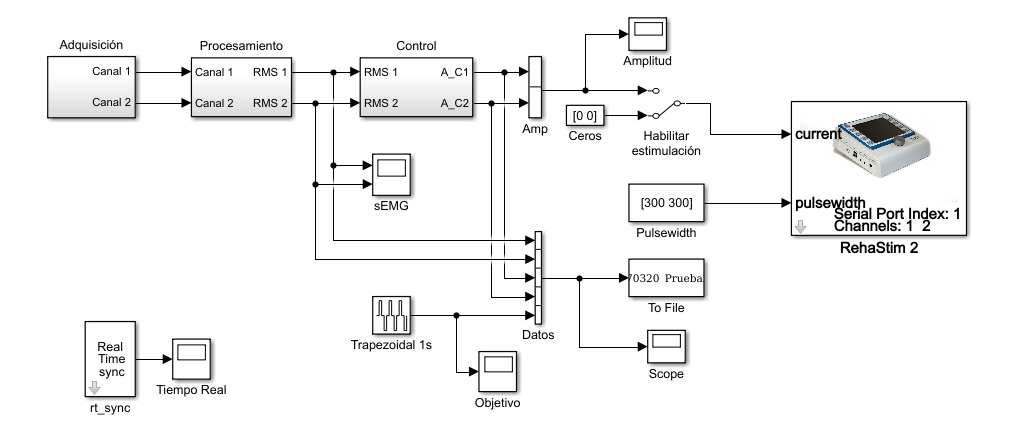
\includegraphics[width=\textwidth]{SistemaCompleto.png}
	\caption{Sistema completo implementado en Simulink.}
	\label{Figura: SisComp}
\end{figure}

Posteriormente, se le indica al sujeto la forma en la que se llevará a cabo la prueba y cómo deberá realizarla. Para esto, al sujeto se le mostrará en un scope una señal trapezoidal con ciclos negativos y ciclos positivos (Figura \ref{Figura: Trapezoidal}), el sujeto deberá realizar el seguimiento de dicha trapezoidal considerando que el ciclo positivo indica apertura de mano completa, mientras que el ciclo negativo indica pinza gruesa completa y que una línea en cero indica descanso. El sujeto deberá realizar una transición entre los movimientos indicados buscando seguir las pendientes de la trapezoidal. Una vez dadas las indicaciones se procede a iniciar la prueba, y a la par el experimentador deberá observar en otro scope la salida del bloque de control, donde se observará si la activación de canales de estimulación eléctrica corresponden a los movimientos que realiza el sujeto (pinza gruesa activa canal 1 de estimulación, apertura de mano activa canal 2 de estimulación, y descanso no activa algún canal de estimulación).

%Trapezoidal
\begin{figure}
	\centering
	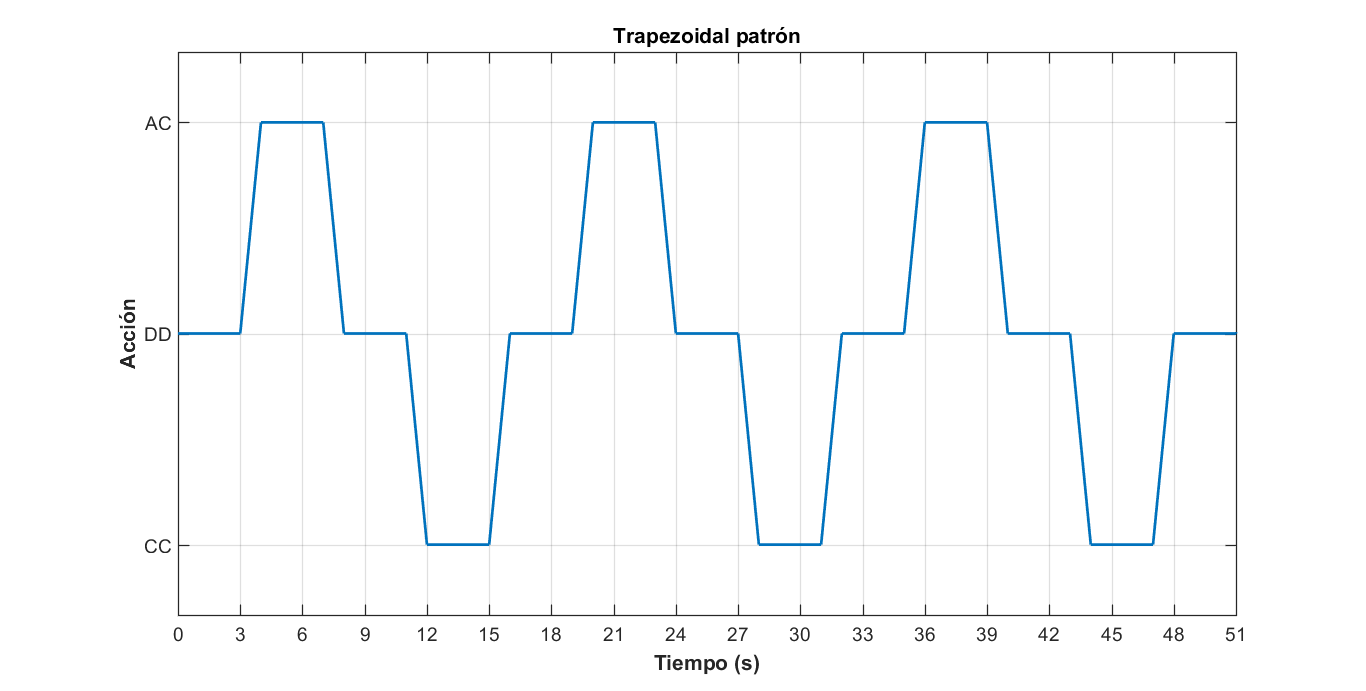
\includegraphics[width=\textwidth]{Trapezoidal.png}
	\caption[Señal trapezoidal objetivo]{Segmento de señal trapezoidal objetivo utilizada para la prueba en línea y tarea objetivo. El ciclo positivo indica al sujeto que realice un movimiento de apertura completa (AC), el ciclo negativo indica al sujeto que realice un movimiento de pinza gruesa completa (CC), mientras que el valor en cero indica que realice un descanso (DD).}
	\label{Figura: Trapezoidal}
\end{figure}

\newpage
\subsection{Tarea objetivo}
Esta prueba final utiliza los mismos parámetros e indicaciones que en la prueba de validación en línea, sin embargo, para esta prueba se aplica estimulación eléctrica al brazo afectado del sujeto, por lo que el switch \emph{Habilitar estimulación} se encuentra conectado la salida del bloque \emph{Control}, y además, el tiempo de término de la simulación se configura a 180 s.

En esta prueba se busca medir el tiempo de retardo que existe entre el inicio del movimiento en la mano sana y el inicio del movimiento en la mano afectada. Para poder realizar esto se almacenan todos los datos de las señales involucradas en el sistema (canales de registros de sEMG, canales de estimulación eléctrica y señal patrón trapezoidal), y posterior a la finalización de la prueba se realiza un análisis manual en MATLAB donde se determina el tiempo de retardo existente para cada movimiento, y se obtiene el promedio del retardo de todas las repeticiones realizadas para obtener un retardo global de la sesión.


%Se diseñó un sistema basado en una combinación de máquina de estados finitos con un control lineal. El sistema requiere de un proceso de calibración previa donde se obtienen 8 umbrales tras la repetición de 4 movimientos, dos umbrales corresponden a los valores RMS promedio de los dos canales de adquisición a lo largo de la tarea \emph{cierre de mano ligero}, otros dos corresponden a los valores RMS promedio de la tarea \emph{cierre de mano completo}, mientras que los 4 restantes corresponden a los valores RMS promedio de las tareas \emph{apertura de mano ligera} y \emph{apertura de mano completa}. Además, tras la calibración se obtiene también un factor denominado \emph{detector de movimiento}, el cual se obtiene tras calcular la diferencia promedio entre los canales de adquisición a lo largo de la tarea de apertura de mano. Adicionalmente se realiza una calibración de la estimulación eléctrica, la cual utiliza el sistema de colocación de electrodos de estimulación descrito en \cite{AnaMartin2019}, donde se obtiene los valores en amplitud de los umbrales motores y funcionales de las tareas de apertura y cierre de mano.
%
%El detector de movimiento se utiliza para realizar el control por máquina de estados finitos (Figura \ref{Figura: FSM_Control}), la cual consisten en determinar si la diferencia de amplitudes entre canales ha pasado el valor del detector de movimiento, si es así, el control prosigue con la tarea de apertura de mano, en caso contrario, el control procede a la tarea de cierre de mano.
%
%\begin{figure}[htbp]
%	\centering
%	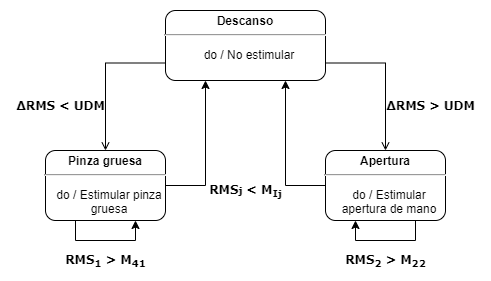
\includegraphics[scale=0.9]{FSM_Control.png}
%	\caption[FSM para control]{Máquina de estados finitos encargada de la detección de movimiento e inicio del control lineal.}
%	\label{Figura: FSM_Control}
%\end{figure}
%
%Dentro del control de cada tarea, se utilizan los umbrales de las tareas ligeras para realizar la activación del control lineal, el cual modula la amplitud de la corriente eléctrica, del canal asociado al movimiento detectado, utilizando la recta descrita por la Ecuación \ref{Ecu: Mapeo}, donde $A$ representa la amplitud que inyectará el estimulador eléctrico, $A_{max}$ es el umbral funcional de estimulación eléctica, $A_{min}$ es el umbral motor de estimulación eléctica, $D$ representa el valor RMS actual, mientras que $D_{max}$ y $D_{min}$ representan los umbrales RMS de la tarea completa y ligera del canal asociado al movimiento detectado (canal 1 para cierre de mano y canal 2 para apertura de mano). Adicionalmente se aplica la función máximo entero a la recta debido a que el dispositivo de estimulación eléctrica sólo admite valores enteros, y también se aplica un criterio de saturación de corriente eléctrica para evitar que tras una contracción muscular muy fuerte se genere un valor de amplitud de corriente eléctrica dañino para el sujeto.
%
%%Ecuación mapeo lineal
%\begin{equation}
%	A = \frac{A_{max} - A_{min}}{D_{max} - D_{min}}(D - D_{min}) + A_{min}
%	\label{Ecu: Mapeo}
%\end{equation}

%\section{Tarea objetivo}
%{\color{red}INCLUIR TAREA OBJETIVO DE ENTRENAMIENTO CON TRAPEZOIDAL EN LÍNEA}
